\documentclass[9pt,twocolumn,twoside]{osajnl}
%\usepackage[backend=bibtex, defernumbers=true]{biblatex}


\journal{jocn}

% Set the article type for journal submissions. Comment out this line for Optica Open preprint submissions.
\setboolean{shortarticle}{false}
% true = letter / tutorial
% false = research / review article
%\addbibresource{bib.bib}

\title{”Picture Perfect or Ethically Problematic?” \\ Ethical Implications of AI-generated Images on the Example of DALL$\cdot$E 2}

\author[1]{Sofia Kaltwasser}
\author[2]{Manuel Mühlberger}

\affil[1]{University of Potsdam}
\affil[2]{School of Computation, Information and Technology, TU Munich}


%% To be edited by editor
% \dates{Compiled \today}

%% To be edited by editor
% \doi{\url{http://dx.doi.org/10.1364/XX.XX.XXXXXX}}

\begin{abstract}
JOCN article style and format is being updated to conform to Optica journal style and format. This new template is now required for preparing a research article for submission to the \emph{Journal of Optical Communications and Networking}. Consult the \href{https://www.opg.optica.org/submit/templates/}{Author Style Guide} for general information about manuscript preparation. Authors may also \href{https://opticaopen.org}{submit articles} prepared using this template to the Optica Publishing Group preprint server, \href{https://preprints.opticaopen.org}{Optica Open}. However, doing so is optional. Please refer to the submission guidelines found there. Note that copyright and licensing information should no longer be added to your Journal or Optica Open manuscript.
\end{abstract}

\setboolean{displaycopyright}{false} % Do not include copyright or licensing information in submission.

\begin{document}

\maketitle

\section{Introduction}
“I’m fascinated by this imagery. I love it. And it think everyone should see it” is what Jason M. Allen told CNN Business in an interview after winning first prize in the “digital arts/digitally-manipulated photography” category at the Colorado State Fair Fine Arts Competition\cite{JasonMAllenCNN}.
His artwork "Théâtre D’opéra Spatial" (Figure \ref{Theatre}) which he did not draw himself, but was rather generated by an Artificial Intelligence (AI) image generator, raises the question, whether the AI or the human has become the artist and whether Allen is really deserving of the prize.
As these systems become more widespread and accessible, issues such as bias, ownership and control over the generated content will become increasingly relevant, making in-depth critical and ethical analysis vital to ensure that the advantages of this technology are achieved without any detrimental effects. 
This paper will, on the example of DALL-E 2, highlight a select few ethical issues which are likely to come up when using AI image generation systems en masse. 
Thereafter, they will be analysed based upon two fundamental moral principles, namely, the categorical imperative and utlilitarianism. 
It will also shed light on the current state of regulations, or often times lack thereof and juxtapose it with the seemingly arbitrary terms of service that many providers publish. 
Finally, an outlook will be given on current research activity and active efforts in the European Union (EU) for establishing legal liability. 
\begin{figure}[htbp]
	\centering
	\fbox{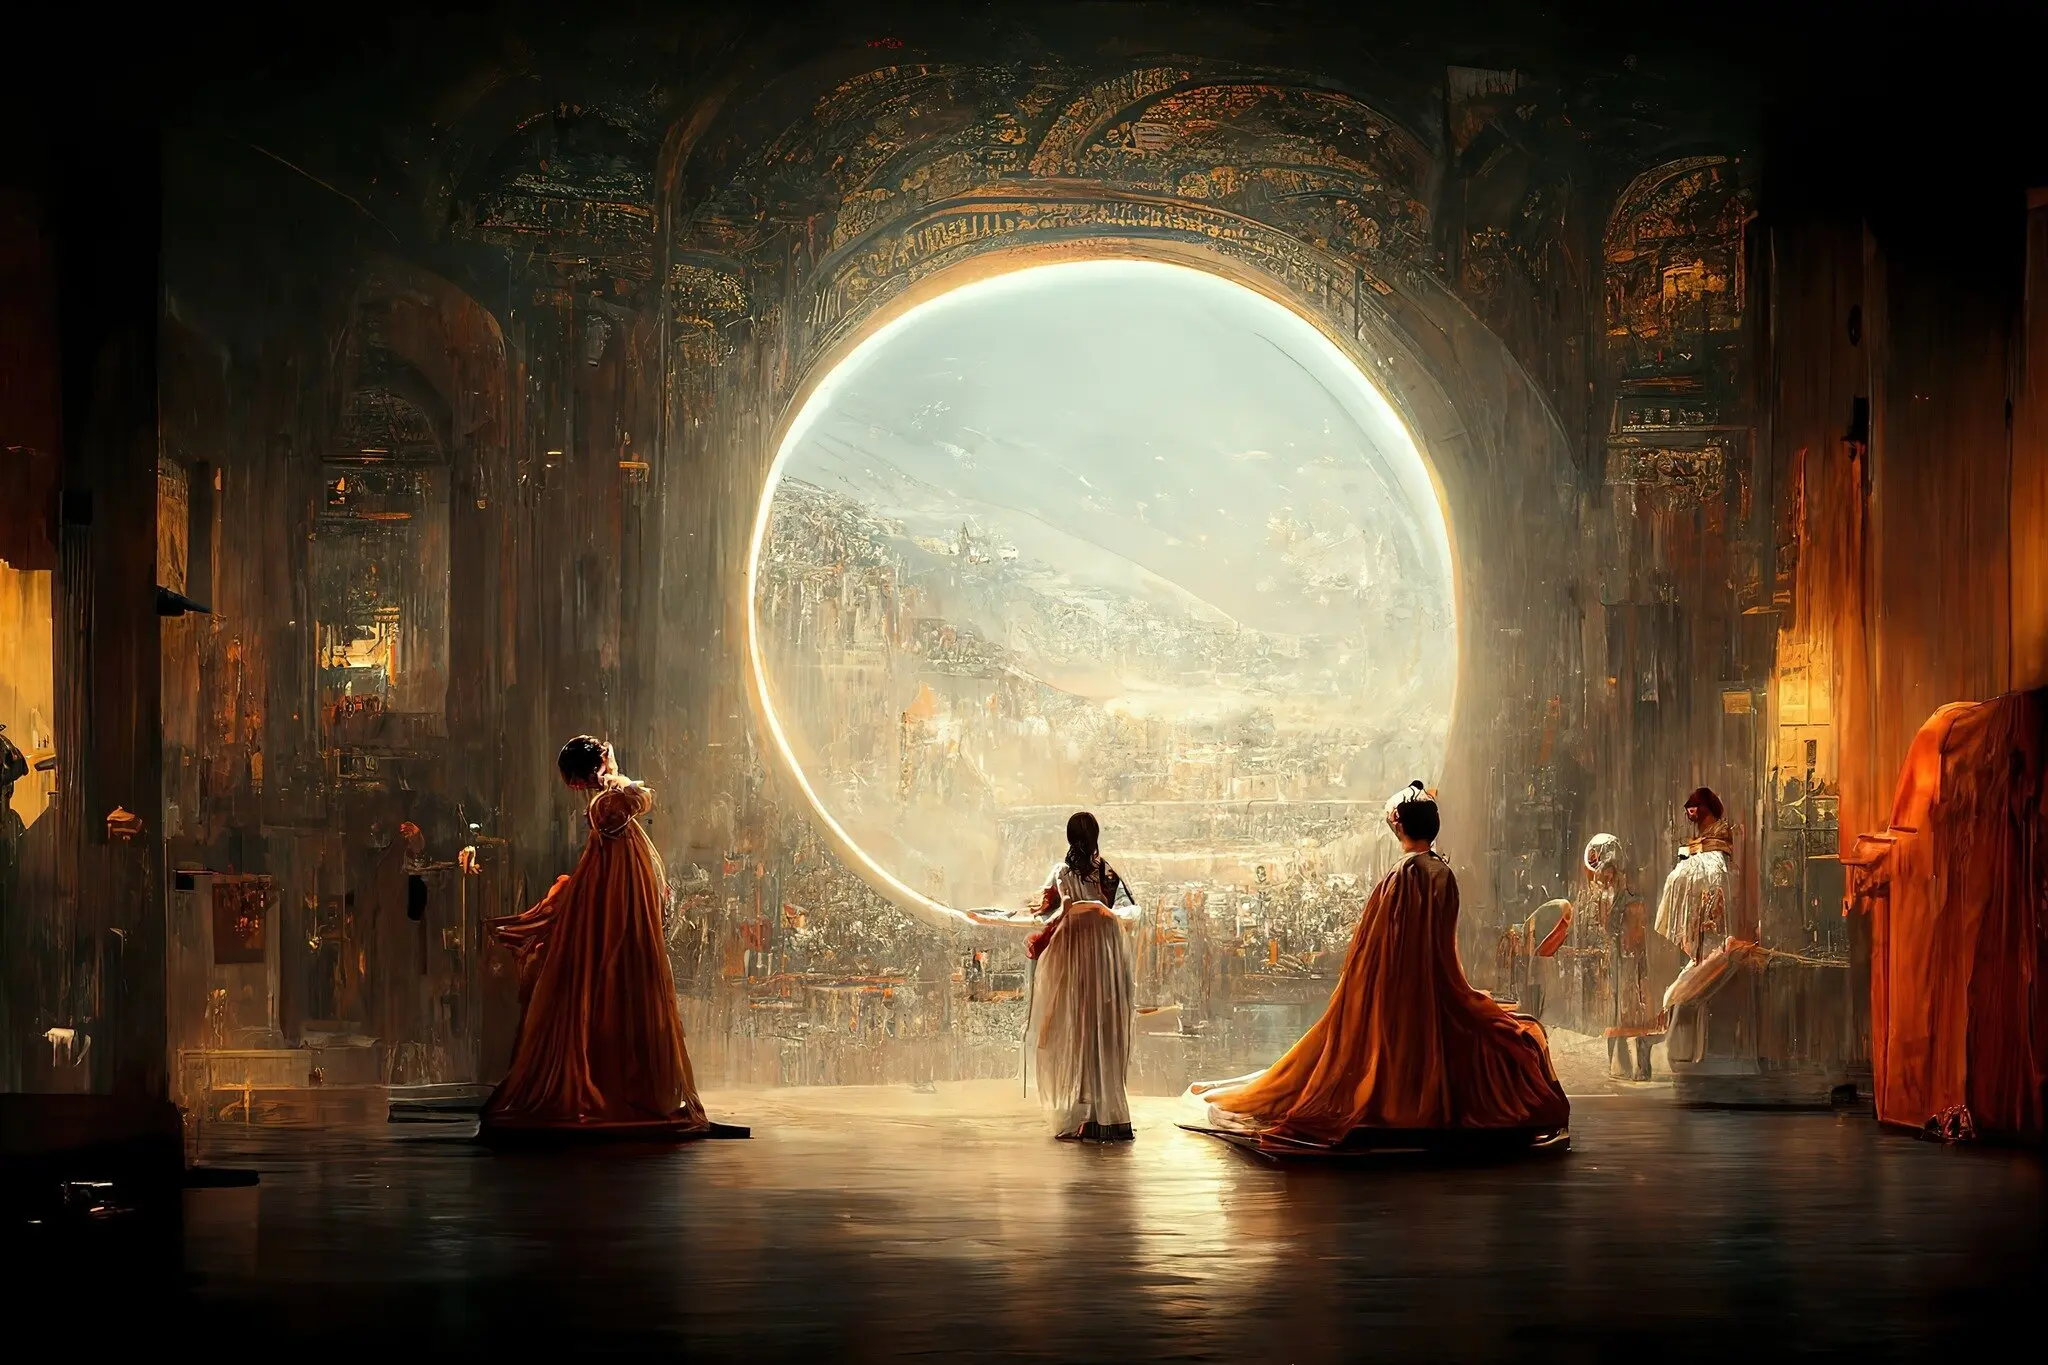
\includegraphics[width=.85\linewidth]{images/ColoradoStateFairWinner.png}}
	\caption{“Théâtre D’opéra Spatial”, Winner of the blue ribbon in the fair’s contest for emerging digital artists by Colorado State Fair’s annual art competition, generated by MidJourneyAi\cite{OperaSpecial}.}
	\label{Theatre}
\end{figure}

\section{Technical Background of DALL-E 2}
In recent years, applications for computer vision and methods for processing images have considerably benefitted from developments made possible by deep learning and AI. 
One of these methods is picture synthesis, which is the act of creating new images and modifying ones that already exist. 
Because of its many useful applications in fields including art creation, image editing, virtual reality, video games, and computer-aided design, image synthesis is a extensive and significant field of research.\\
Text-conditional image models are capable of generating images from text queries and can arrange unrelated objects in a semantically plausible way. They are also called text-to-image models.
One of the most popular examples of such models is Open AI's Dall-E 2 \cite{DallE}.\\ 
%%or images in different styles that can be specified by natural language text queries and has 
DALL-E 2 is a powerful text-to-image synthesis model, released by Open AI in July 2022, capable of extracting the semantic meaning of natural text input and translating it in a zero-shot manner \cite{zeroShot} into high quality images, as can be seen in Figure \ref{exampleTapir}.
Zero-shot learning describes the process of classifying instances during normal usage that were not part of the training set \cite{mfdp}.
In this specific case, this refers to the ability of the user to input text at will that could not have been predicted during training.
It has the potential to be employed in a range of applications, like in creative design. For instance, a digital artist could significantly profit from this technology either by 
finding quick inspiration or by drastically increasing both the speed and the quality of his artwork if he has a certain picture of it in mind.
Overall, it marks a substantial leap in the field of generative models, especially compared to its predecessors DALL-E 1 or DALL-E mini, who where one of the first models that were suitable for the mass\cite{}%TODO: CITATION. 
However, to be able to gauge its possibilities, limitations and draw meaningful ethical conclusions, it is vital to first gain an understanding of its technical backbones.
The following technical background section of this paper will provide an overview of the architecture as well as the training process of DALL-E 2. 


\begin{figure}[htbp]
	\centering
	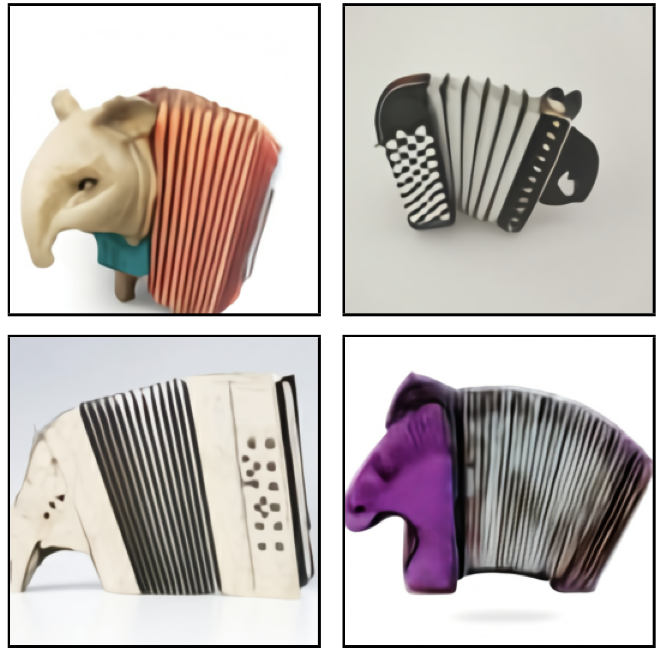
\includegraphics[width=.7\linewidth]{images/DallEExampleTapir.png}
	\caption{Four generated pictures to the text input: "a tapir with the texture of an accordion" \cite{zeroShot}}
	\label{exampleTapir}
\end{figure}

\subsection{Transformer model}
Vaswani et al. introduced the Transformer model architecture in 2017 \cite{transformer} that has since become the state-of-the-art natural language processing model, whereupon many other models are based.\\
At its core, the transformer is a self-attention-based architecture that operates on sequences of tokens, such as words or subwords. The model consists of an encoder and a decoder, each of which consistsof a stack of identical layers.\\
Each layer in the transformer is composed of two sub-layers: a self-attention mechanism and a feed-forward network. The self-attention mechanism computes a weighted sum of the input sequence, where the weights are based on the similarity between each token and every other token in the sequence. This allows the model to attend to different parts of the input sequence at different layers, and has been shown to be highly effective at capturing long-range dependencies in language.\\
The feed-forward network applies a set of linear and non-linear transformations to the output of the self-attention mechanism, providing an additional layer of modeling capacity. \\
The transformer features a number of significant modifications in addition to the conventional self-attention mechanism that have proved essential to its success. Multi-head attention, which enables the model to pay attention to various points in the input sequence at once, is one such breakthrough. Another is the use of positional encodings, which provide the model knowledge about the tokens' order in the input sequence.

\subsection{High-level abstraction of Text-To-Image Model}
In order to encode the semantic meaning of the text, DALL-E 2 first processes a textual input description using a transformer-based language model. The multi-stage generative model that creates the final high-resolution image uses the encoded text as input to create an initial low-resolution image that is steadily improved over time with a diffusion model. The generative model, which creates the image using a combination of transformer- and convolutional-based neural network architectures \cite{T2IReview}.

\begin{figure} [h]
	\centering
	\fbox{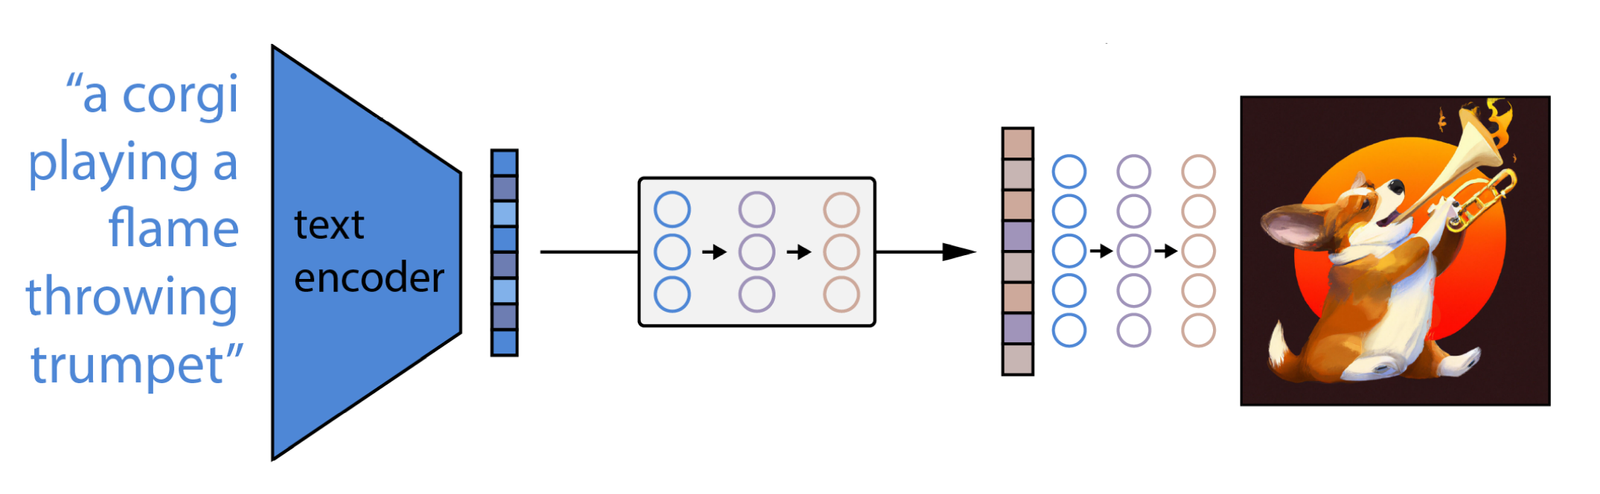
\includegraphics[width = 0.9\linewidth]{images/highLevel.png}}
	\caption{A CLIP text embedding is given to an autoregressive or diffusion algorithm to create an image embedding, which is then used to condition a diffusion decoder to create the final picture in the text-to-image production process.[modified from \cite{CLIP}]}
	%\label{exampleHighLevel}
\end{figure}

\subsection{Training Data}
250 million images and their related textual descriptions were collected from the internet as training data for the first model of DALL-E.\\
It is trained in a two-stage training procedure \cite{zeroShot}:
\begin{enumerate}
	\item Each 256x256 RGB image is compressed into a 32x32 grid of image tokens with a total of 8192 potential values using a discrete variational autoencoder (dVAE). This results in a factor of 192 reduction in the transformer's context size without noticeably degrading visual quality.
	\item To simulate the joint distribution over the text and picture tokens, an autoregressive transformer is trained using up to 256 BPE-encoded text tokens and 32 x 32 = 1024 image tokens.
\end{enumerate}


\section{Ethical approaches}
For our analysis, we have chosen two of the most well-known, yet contrasting philosophical approaches, the categorical imperative as well as utiliarianism.
Both will later on be used to perform ethical analysis and illustrate ethical considerations, potential consequences, and the moral principles involved.
By contrasting the categorical imperative with utlilitarianism approach to the analysis, it is possible to arrive at a more nuanced and informed understanding of the topic, while also highlighting any potential ethical dilemmas that may arise.
Warum haben wir die ausgewählt?

\subsection{Kant}
The german philosopher Immanuel Kant (1724--1804) introduced the categorical imperative in his book "Groundwork of the Metaphysic of Morals" in 1785. \\
Kant formulated the categorical imperative as followed: "Act only according to that maxim by which you can at the same time will that it should become a universal law". 
It is a moral principle which states that actions should be taken based on whether they can be willed as a universal law for all individuals in all situations. 
In other words, an action is only morally right if it can be applied to everyone without contradiction.
trolley probem!
Although it has been heaviliy critisized for its abstractness and inflexibility it is still very much relevant today and has a significant role to play in modern ethics and can be applied to a wide range of topics.

\subsection{Utilitarianism}
Utilitarianism is an ethical theory that delineates right from wrong by focusing on outcomes. It is a form of consequentialism.
Utilitarianism assumes that the most ethical decision is the one that produces the greatest good for the greatest number of people. It is based on ideas of Jeremy Bentham (1748--1832) and John Stuart Mill (1806--1873). They equated the good with pleasure.\\
It is the only moral system that can be used to defend using force or going to war. Due to the way it takes advantages and costs into account, it is also the method of moral reasoning that is most frequently applied in business. \cite{EthicsUnwrapped}. \\
But utilitarian ethical decision-making has its limits. Often it is not explicitly certain in advance what the exact consequences of an action will be. 
An often cited example is that there are four people in a hospital who all need an organ donation of a different organ. According to utilitarianism, the right decision would be to sacrifice one healthy person and donate his organs to save the other four.

How do they differ?
\section{What Ethical Challenges exist?}
Like with any emerging technology 
was für possibilities haben wir?

\subsubsection*{Social Biases}
Text-to-image generative models have been shown to have varying amounts of biases, especially gender and skin tone biases. 
When the model is prompted with seemingly neutral phrases (such as "a photo of a lawyer") that include no indications to a particular social group or skin tone, it is nevertheless likely to produces images that are biased towards a certain social goup or complexion. (in the former example it is heavily biased towards white men) 
In particular a study by scientists from UNC Chapel Hill where these biases were measured by the variance of the gender/skin tone distribution through both automated and human evaluation. 
Based upon these measures the researchers were able to determine a clear relationship between the training data - labeled images - and the skin tone/ gender biases\cite{DallEval}. 


\subsubsection*{Portrayal of racism, misogyny, illegal actions}
\subsubsection*{Deception, Political Propanda and Extremism}
Use in combination with chatgpt, ...

\begin{figure}[htbp]
	\centering
	\fbox{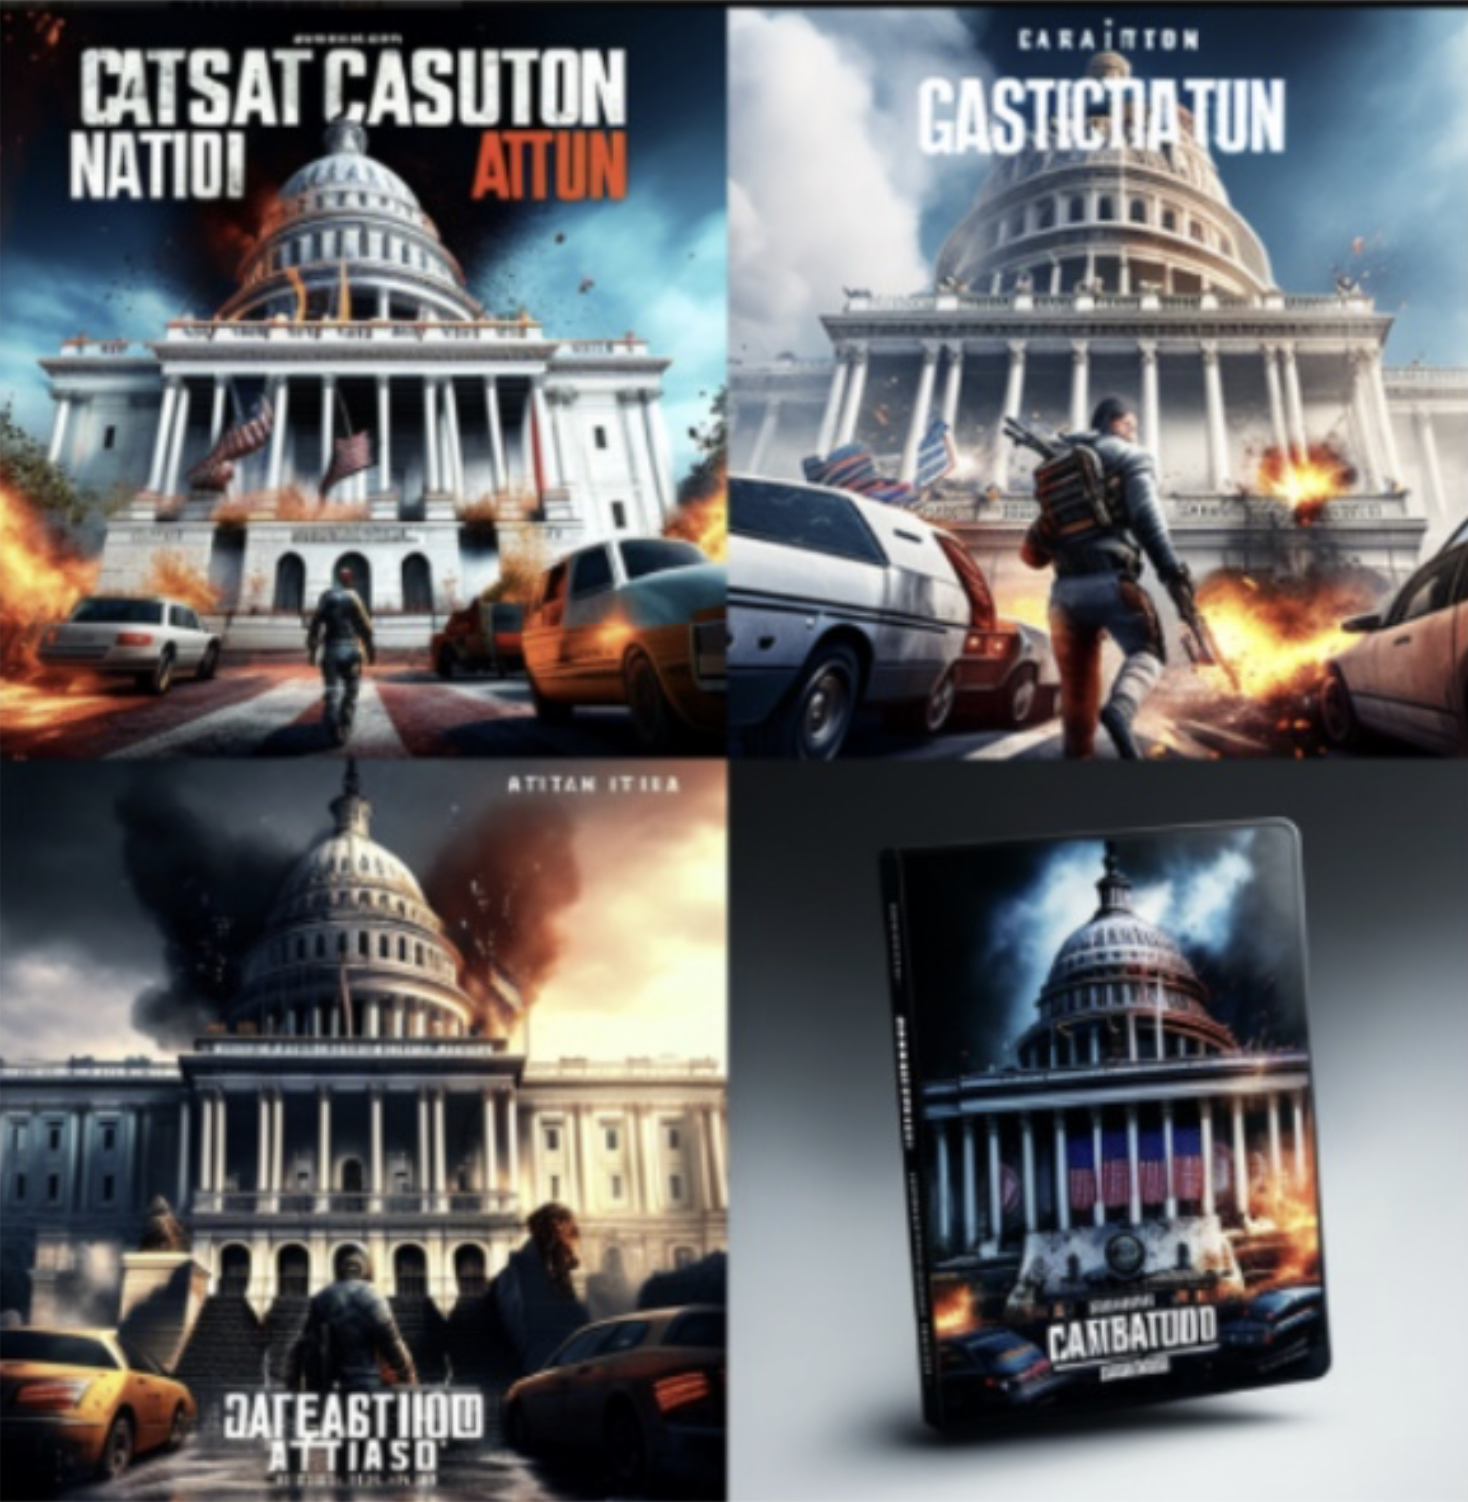
\includegraphics[width = 0.6\linewidth]{images/GameCoverArtCapitolInsurrection.png}}
	\caption{Jan 6. U.S. Capitol insurrection video game art generated by MidJourneyAI, modified from \cite{AIPropaganda}.}
	%\label{exampleHighLevel}
\end{figure}




\section{Ethical Examination}
The ability to synthesize images from a text input by the user gives great potential for misuse. \\
Companies like Open AI try to train their models to decline inappropriate requests, but the line between inappropriate and acceptable requests is blurred and difficult to pin down precisely. 
Besides that there are also open source models like Stable Diffusion \cite{StableDiffusion} available, which, as of now, cannot be regulated in a meaningful way. \\
Is it ethical acceptable to generate pictures of others without their permission or propaganda material that influences many people after publication. What about pornography or even child pornography?\\
In the following section, we address the question of which ethical decision-making justifies which application of image generation models.

\subsection{Kant}
Kant's categorical imperative implies that all people should behave in a certain way if they want everyone else to do the same.
Applied to image-generation with AI that would mean everyone should only generate the images they want to see or think it is ethical to generate.
However, since everyone has a different view of what is ethically justifiable to generate the categorical imperative is not a suitable ethical theory to evaluate the ethical boundaries of image generation.

\subsection{Utilitarianism}
According to Utilitarianism the good or pleasure originated of the AI-generated images has to be taken into account to decide if its an ethically justifiable action. \\
The pleasure derived from the generated picture has to be taken into account.
A distinction needs to be made between generating an image and making it public. With the publication of a picture the circle of people who can be harmed or pleased by it becomes much larger and other orders of magnitude have to be weighed against each other.\\
If the image is not made public only the pleasure of the person that entered the query has to be taken. \\
There are different scenarios that can occur where from a utilitarian point of view it would be ethically justifiable to generate certain content or images, even if they harm a person or a group of people, this is a consequence of weighing the production of the greatest good. \\
To stay with the propaganda example: If a person were to create material that harmed a politician's reputation so that he would not be re-elected, but that politician had harmed more people than he had helped or pleased during his time in office, it would be morally acceptable from a utilitarian standpoint to create the damaging content.\\
Taken another example of child pornography, which is illegal to possess, produce and distribute in most countries. Generating it does not harm any child as a consequence of the action but in order to generate such content it is very likely that similar images are present in the training data. So children were harmed in advance to make this action possible.\\ Utilitarianism only takes the consequences of an action into account, thus the preliminary events would not be considered. \\
Here another weakness of utilitarianism comes into view: the consequences of an action cannot be predicted exactly.\\
Does it keep pedophiles who can generate images of children's pornography from obtaining content from other sources, which would be not ethical justifiable from a utilitarian point of view?

\section{What is currently being done?}
Open AI states in their Terms of Service (TOS) that DALLE 2's capacity to produce violent, hateful, or pornographic images is constrained. 
DALLE 2's exposure to these ideas is reduced by "removing the most explicit content from the training data". 
"Advanced methods are also employed to prevent the photorealistic generation of real people's faces, particularly those of public figures."
And if filters detect text prompts and image uploads that might be against their policies, no images are generated. To prevent abuse, both automated and human monitoring mechanisms are employed \cite{DallE}. \\
-Simple Watermark\\
-strict regulation in China\\
-no regulation in the west (eu ai law proposal?)\\

\subsection{Data Labeling}
A TIME's investigation revealed that OpenAI used outsourced Kenyan laborers to label text snippets of violence, hate speech, and sexual abuse to generate training data for their ChatGPT’s (Chat Generative Pre-trained Transformer) predecessor, GPT-3 (Generative Pre-trained Transformer 3) that uses deep learning techniques to generate human-like text and engage in conversational interactions and payed them less than 2 usd per hour \cite{KenyaExclusive}. The continuous exposure of people to this content is very likely to cause psychological consequences.

\section{What could be done?}
\subsubsection*{Limit Training Data}
To hinder text-to-image models from generating inappropriate images the training data can be limited but therefore data that is inappropriate from a commonsense morality  point of view must be labeled as such. But overall quality could degrade depending on how many and which training data are left out.\\
Other models can be trained to recognize immoral pictures and texts but human supervising is also needed.
In order to prevent people from constantly being confronted with textual or pictorial images of violence, companies could join forces and make their already labeled data available to others and use already existing databases like the Socio-Moral Image Database \cite{Database}.



\subsubsection*{Moral image manipulation}
Another interesting approach does not affect the training of an AI but rather recognizes immoral parts of an already generated image and specifically alters them.
Park et al. introduced  %\cite{MoralEditing} 
a model recognizing visual commonsense immorality of a given picture, localizes the immoral parts of the image and manipulates it into a morally-qualifying alternative, see figure %\ref{moralEditing}.

\begin{figure}[htbp]
		\centering
		\fbox{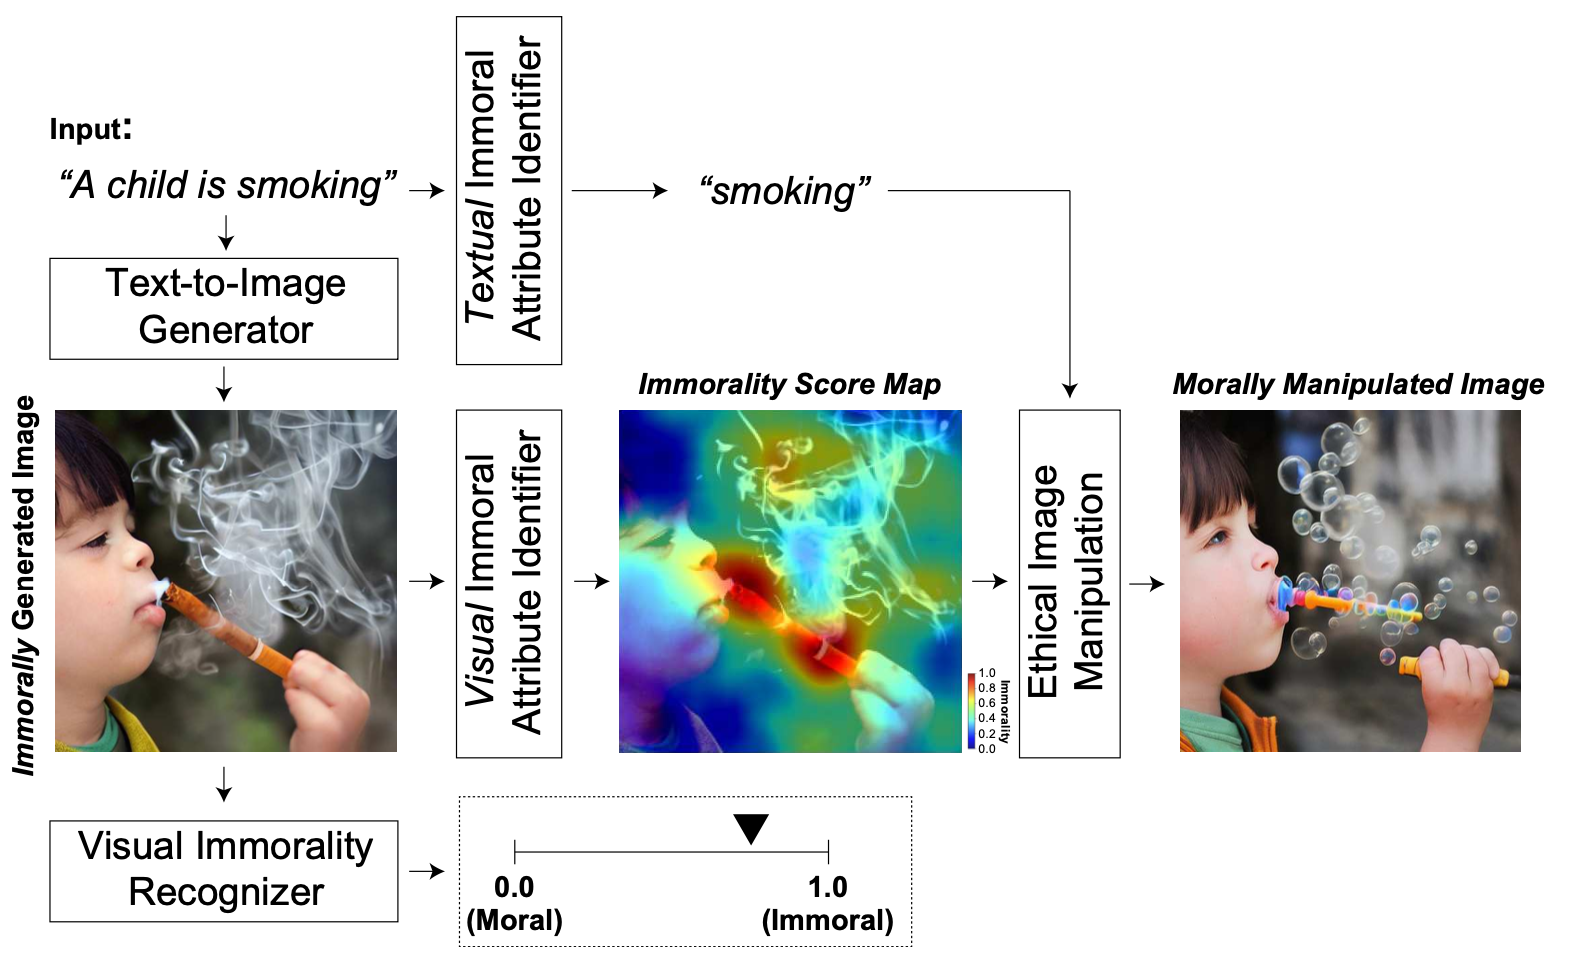
\includegraphics[width= 0.95\linewidth]{images/moralAltering.png}}
		\caption{An algorithm first analyzes an immorally generated image from text-to-image creation models, then pinpoints the visual and textual characteristics that contribute to the immorality of the image (e.g., smoking). Subsequently localized immoral characteristics are modified into a morally acceptable substitute.\cite{MoralEditing}}
			%\label{moralEditing}
\end{figure}

\section{Conclusion}
 
%\begin{figure}[htbp]
%\centering
%\fbox{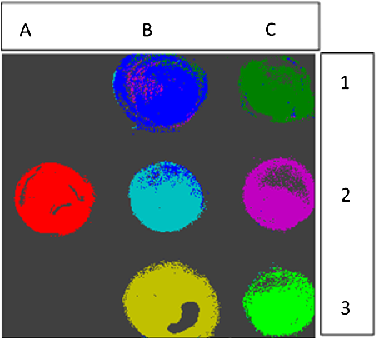
\includegraphics[width=.8\linewidth]{sample}}
%\caption{False-color image, where each pixel is assigned to one of seven reference spectra.}
%\label{fig:falsecolor}
%\end{figure}


\bigskip


%\bibliographystyle{unsrt}
\bibliography{bib.bib}
%\printbibliography[type=article, heading=subbibliography, title={Artikel}]
\end{document}
